\section{用户兴趣表示与匹配的研究}
本章将从用户兴趣的特征作为切入点,对每种特征进行深入分析,提出一套完整的兴趣表示方法。根据第二章中的讨论,兴趣具有最明显的两个特征是关联性和动态性。前者说明的是兴趣概念的关系如同名词之间的关系一样具有同义词、上义词和下义词等,文中提出了一种静态兴趣分类树的模型来充分表示这个特征。后者说明的是用户兴趣会随时间变化而变换,并且分为长期兴趣和短期兴趣,所以文中提出了一种动态兴趣伸展树的模型来解决这一变化的过程。此外,为了使系统能够自动地学习用户的兴趣爱好,以便将来可以为用户推荐兴趣(主题)相似的资源,文中提出了一种学习和推荐的方法来完成这个工作。

\subsection{基于文本主题的兴趣点描述方法}
在正式讨论兴趣树的细节之前,先对文本中涉及兴趣相关的概念进行说明和形式化定义。

给定大小为$V$的词汇表$\mathcal{V}=\{v_1,...,v_V\}$,对于大小为$K$的兴趣全集$\mathcal{I}=\{\vec{in}_1,...,\vec{in}_K\}$,其中$\vec{in}_i~(i\in [1,K])$为第$i$个兴趣点。在本文中,兴趣点的名称$name(\vec{in})$是一个字符串,兴趣点的值$value(\vec{in})$看做是从兴趣变量$\vec{x}$抽样出的一个观测值,兴趣变量$\vec{x}$服从Dirichlet分布,即:
\begin{equation*}
  p(\vec{x}|\vec{\alpha})=Dir(\vec{x}|\vec{\alpha})=\frac{\prod_{i=1}^{V}\Gamma(\alpha_i)}{\Gamma(\sum_{i=1}^{V}\alpha_i)}\cdot \sum_{i=1}^{V}x_i^{\alpha_i-1},~~(\vec{\alpha}=(\alpha_1,...,\alpha_V))
\end{equation*}
可以看出,兴趣点$\vec{in}$是一个$V$维的向量,向量中每个值表示当前词汇对兴趣的权重。因此,对于两个兴趣点$\vec{in}_i$和$\vec{in}_j$\$,它们之间的相似度$d_{i,j}$可以用余弦相似度来衡量:
\begin{equation}
  \label{eq:intsim}
  d_{i,j}=cos(\vec{in}_i,\vec{in}_j)
\end{equation}

要说明的是,这里的兴趣点的表示方式本质上是继承自文本中的主题,在下文没有特别说明的情况下,可以认为兴趣点等价于主题。同时,关于如何估计兴趣变量$\vec{x}$参数的方法就等同于如何在给定的语料库中训练出主题分布$\Phi$。所以,在这一章中,可以默认提取兴趣点的方式都已经存在,重点是如何利用这些兴趣点构建用户的兴趣树。

\subsection{静态兴趣分类树的表示方法}
这一节主要针对兴趣间的关联性问题,对整个兴趣集建立一个描述模型,从而能够展现出兴趣间的关系。从兴趣点的名称来看,这些名称一般为名词,自然而然地想到了兴趣点之间应该是一种层次关系,于是本节提出了用静态兴趣分类树的方式进行描述整个兴趣集。

\begin{figure}
\centering
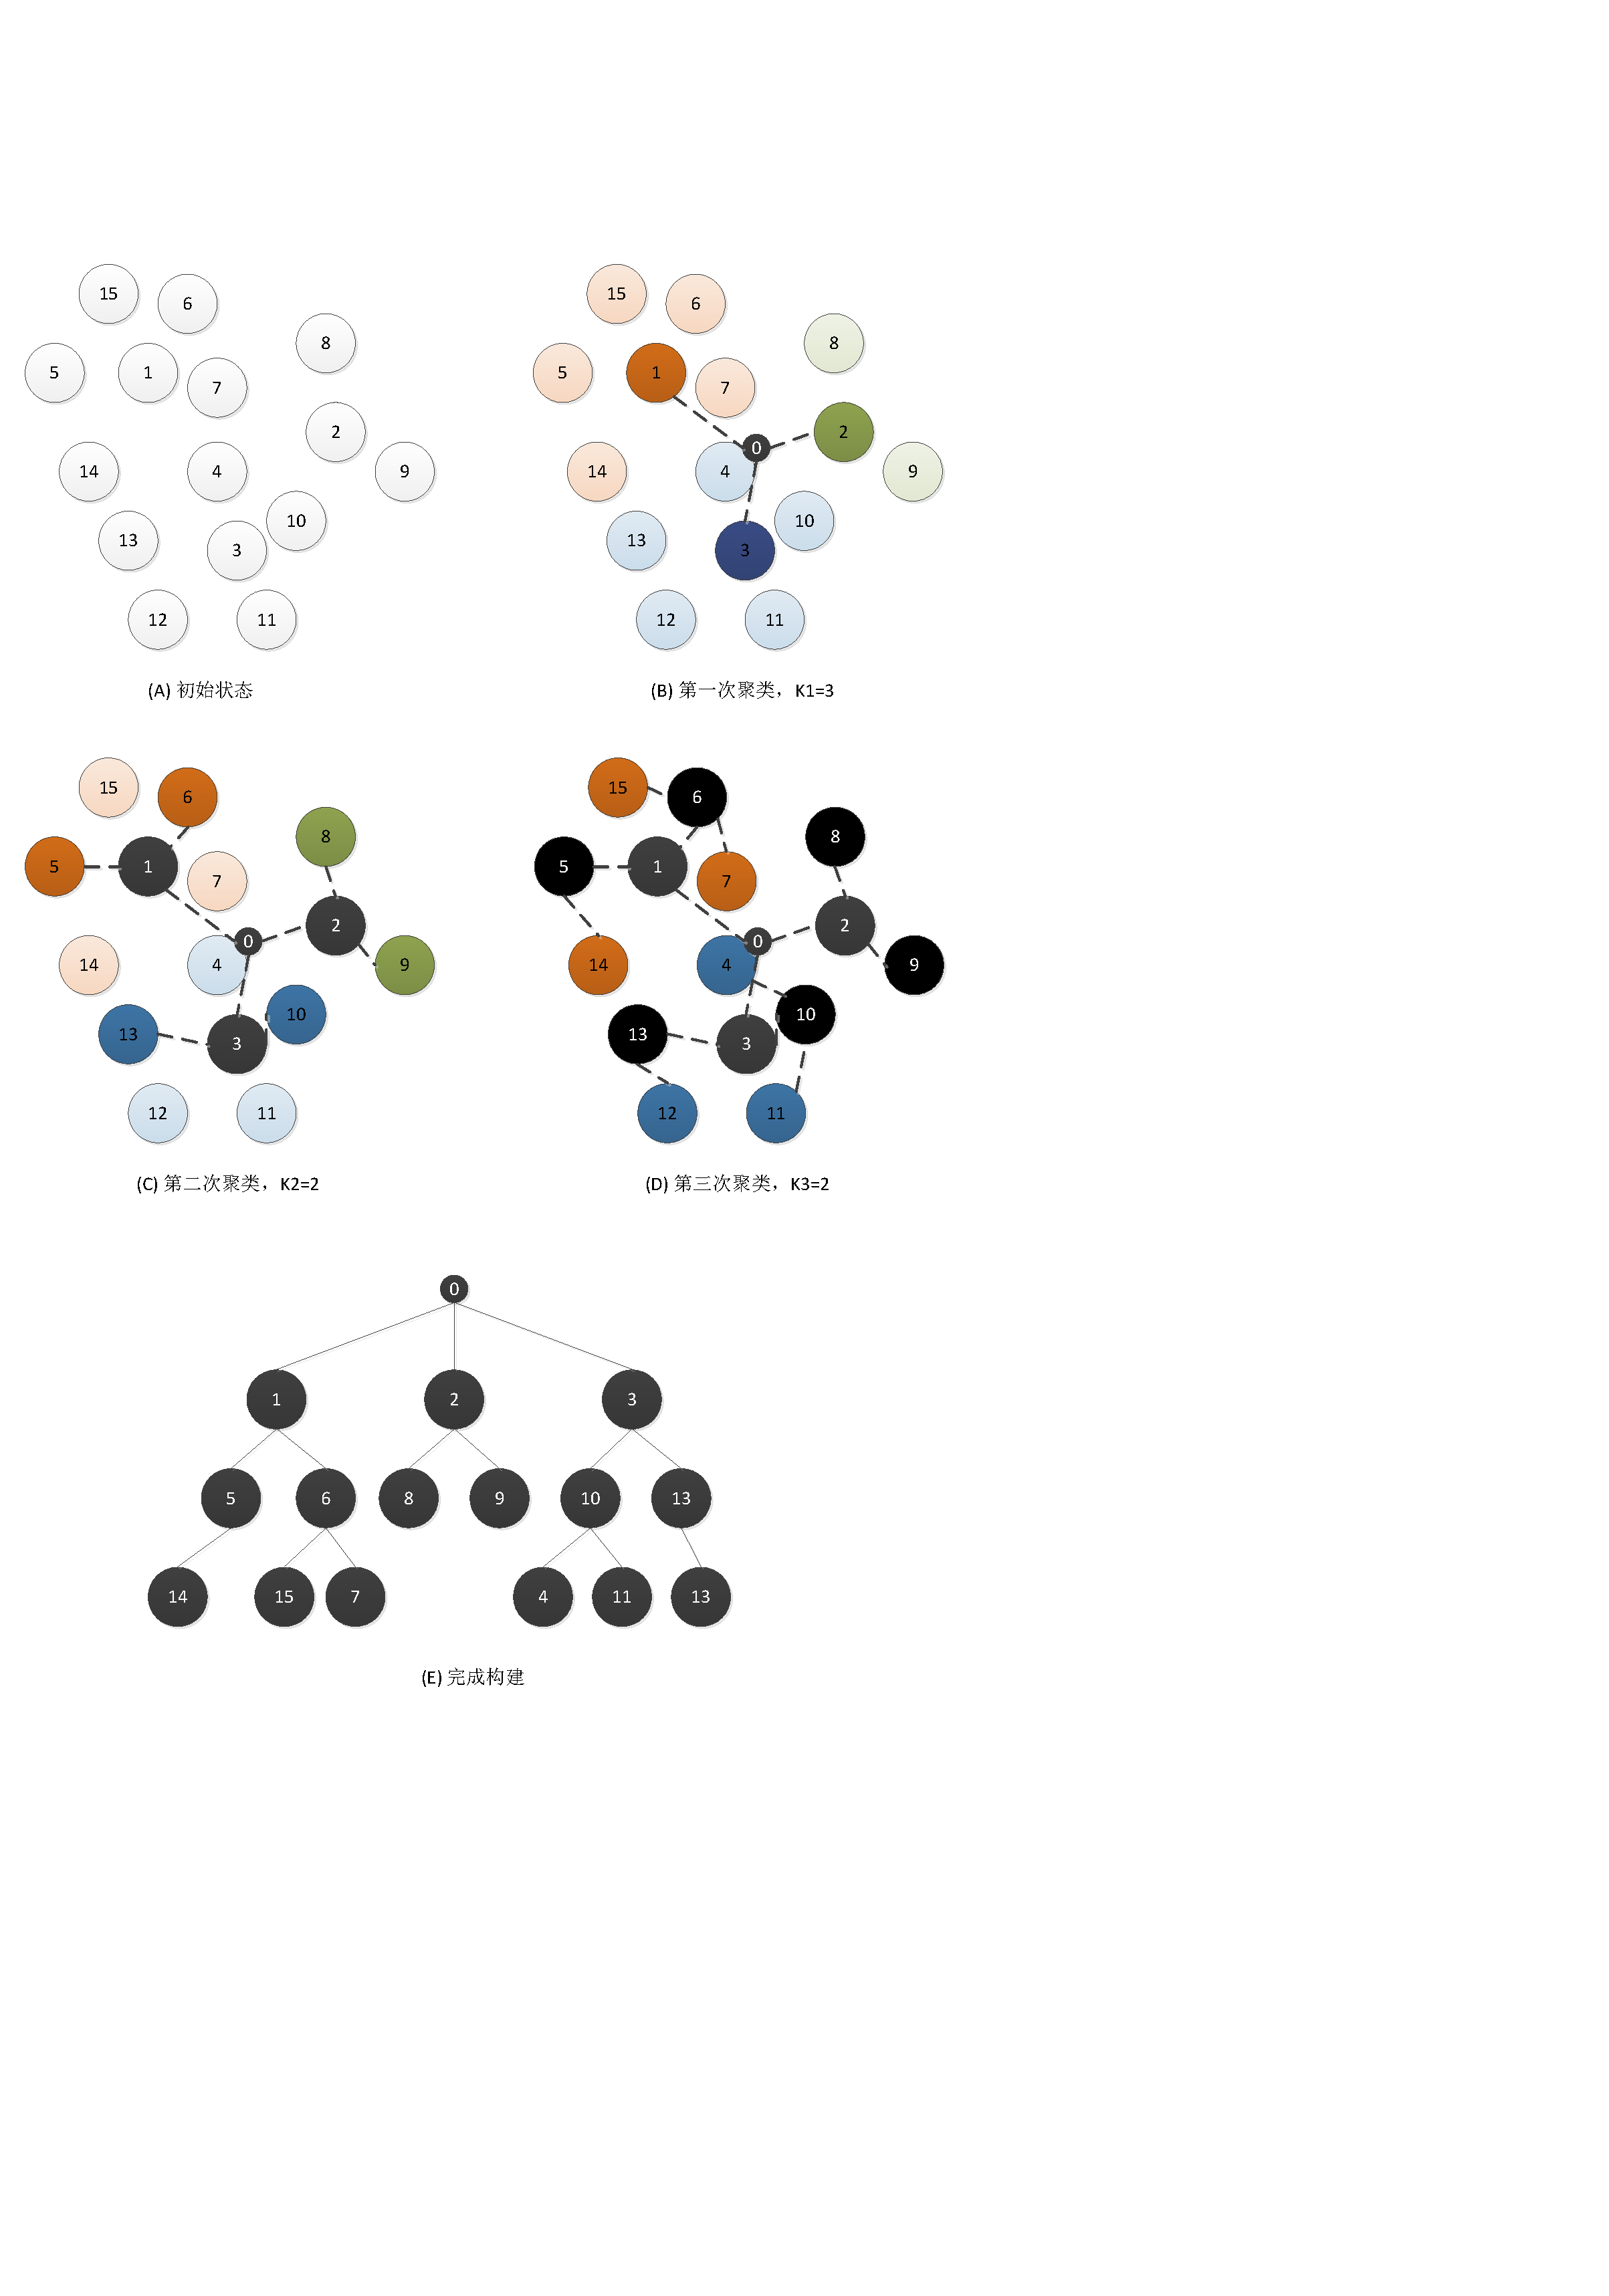
\includegraphics[width=\textwidth]{statictree.pdf}
\caption{基于兴趣余弦相似度的静态兴趣分类树的自动构建示例}
\label{fig:statictree}
\end{figure}

\subsubsection{静态兴趣分类树的构建}
在第二章中提出了几种构建静态兴趣分类树的方法,其中,人工构建法最为精确,但是对于大量的兴趣点时就会很耗时间和精力。相对的是自动构建法,其能够快速自动地对兴趣集合$\mathcal{I}$构建兴趣分类树,但是精确度是一个问题,下面来详细讨论一下基于公式\ref{eq:intsim}计算出来的兴趣相似度为何不能体现出兴趣的层次结构。

首先回顾一下自动构建兴趣分类树的方法,参照图\ref{fig:statictree}中的实例进行详解其每一步的过程:
\begin{enumerate}
  \item 对于初始化状态的兴趣点集合,它们之间可以通过公式\ref{eq:intsim}计算相似度。如图中(A)所示,初始状态一共有15个不同的兴趣点,编号从1至15。
  \item 因为根节点并不表示任何兴趣,所以虚构一个根节点0,所以第一步是构建树中的第二层。如图中(B)所示,先手动给定要聚成3类,那么根据聚类算法(这里假设是K-means)可以分成三个不同颜色的类,其中节点1、2、3分别是三个类的中心,中心的点在兴趣集合中表示该兴趣点涉及的概念和范围更加广泛,因此更适合做该类中其他节点的父节点。最后这三个中心节点与根节点相连,形成树中的第一层。
  \item 第二步是构建树中的第三层。如图中(C)所示,这是给定要在三个类中各自再聚成2类,经过聚类算法实施后,执行和第一步一样的操作。
  \item 第三步是构建树中的第四层。如图中(D)所示,这次依然给定要聚成2类,这时因为各类中的元素已经小于或等于2个,所以在聚类算法结束的时候正好把所有节点都可以连起来。
  \item 第四步对图重画,得到如图(E)中的一个兴趣分类树。由于这个树的结构需要变化的情况十分少,即插入新的兴趣点或删除旧的兴趣点的情况很少发生(至少相对于用户自己的兴趣变化来说),因此称之为静态兴趣分类树。
\end{enumerate}

从上面的过程可以看出,兴趣分类树的构建基础依赖于兴趣点的余弦相似度,树中每一层节点的确定完全依赖于聚类过程中的中心节点,而在树中父节点与孩子节点的实际意义是位于父节点的兴趣点在概念和内容上比处于孩子节点的兴趣点更加宽泛。换句话说,在这个构建的过程中,“宽泛概念”的表现是树中的层次结构,其量化的方法是对“中心节点”的求解,而中心节点的计算又依赖于余弦相似度,因此这里的假设前提是由普通的余弦相似度得到的节点间距离能够反映出层次结构。

\begin{figure}[ht]
\centering
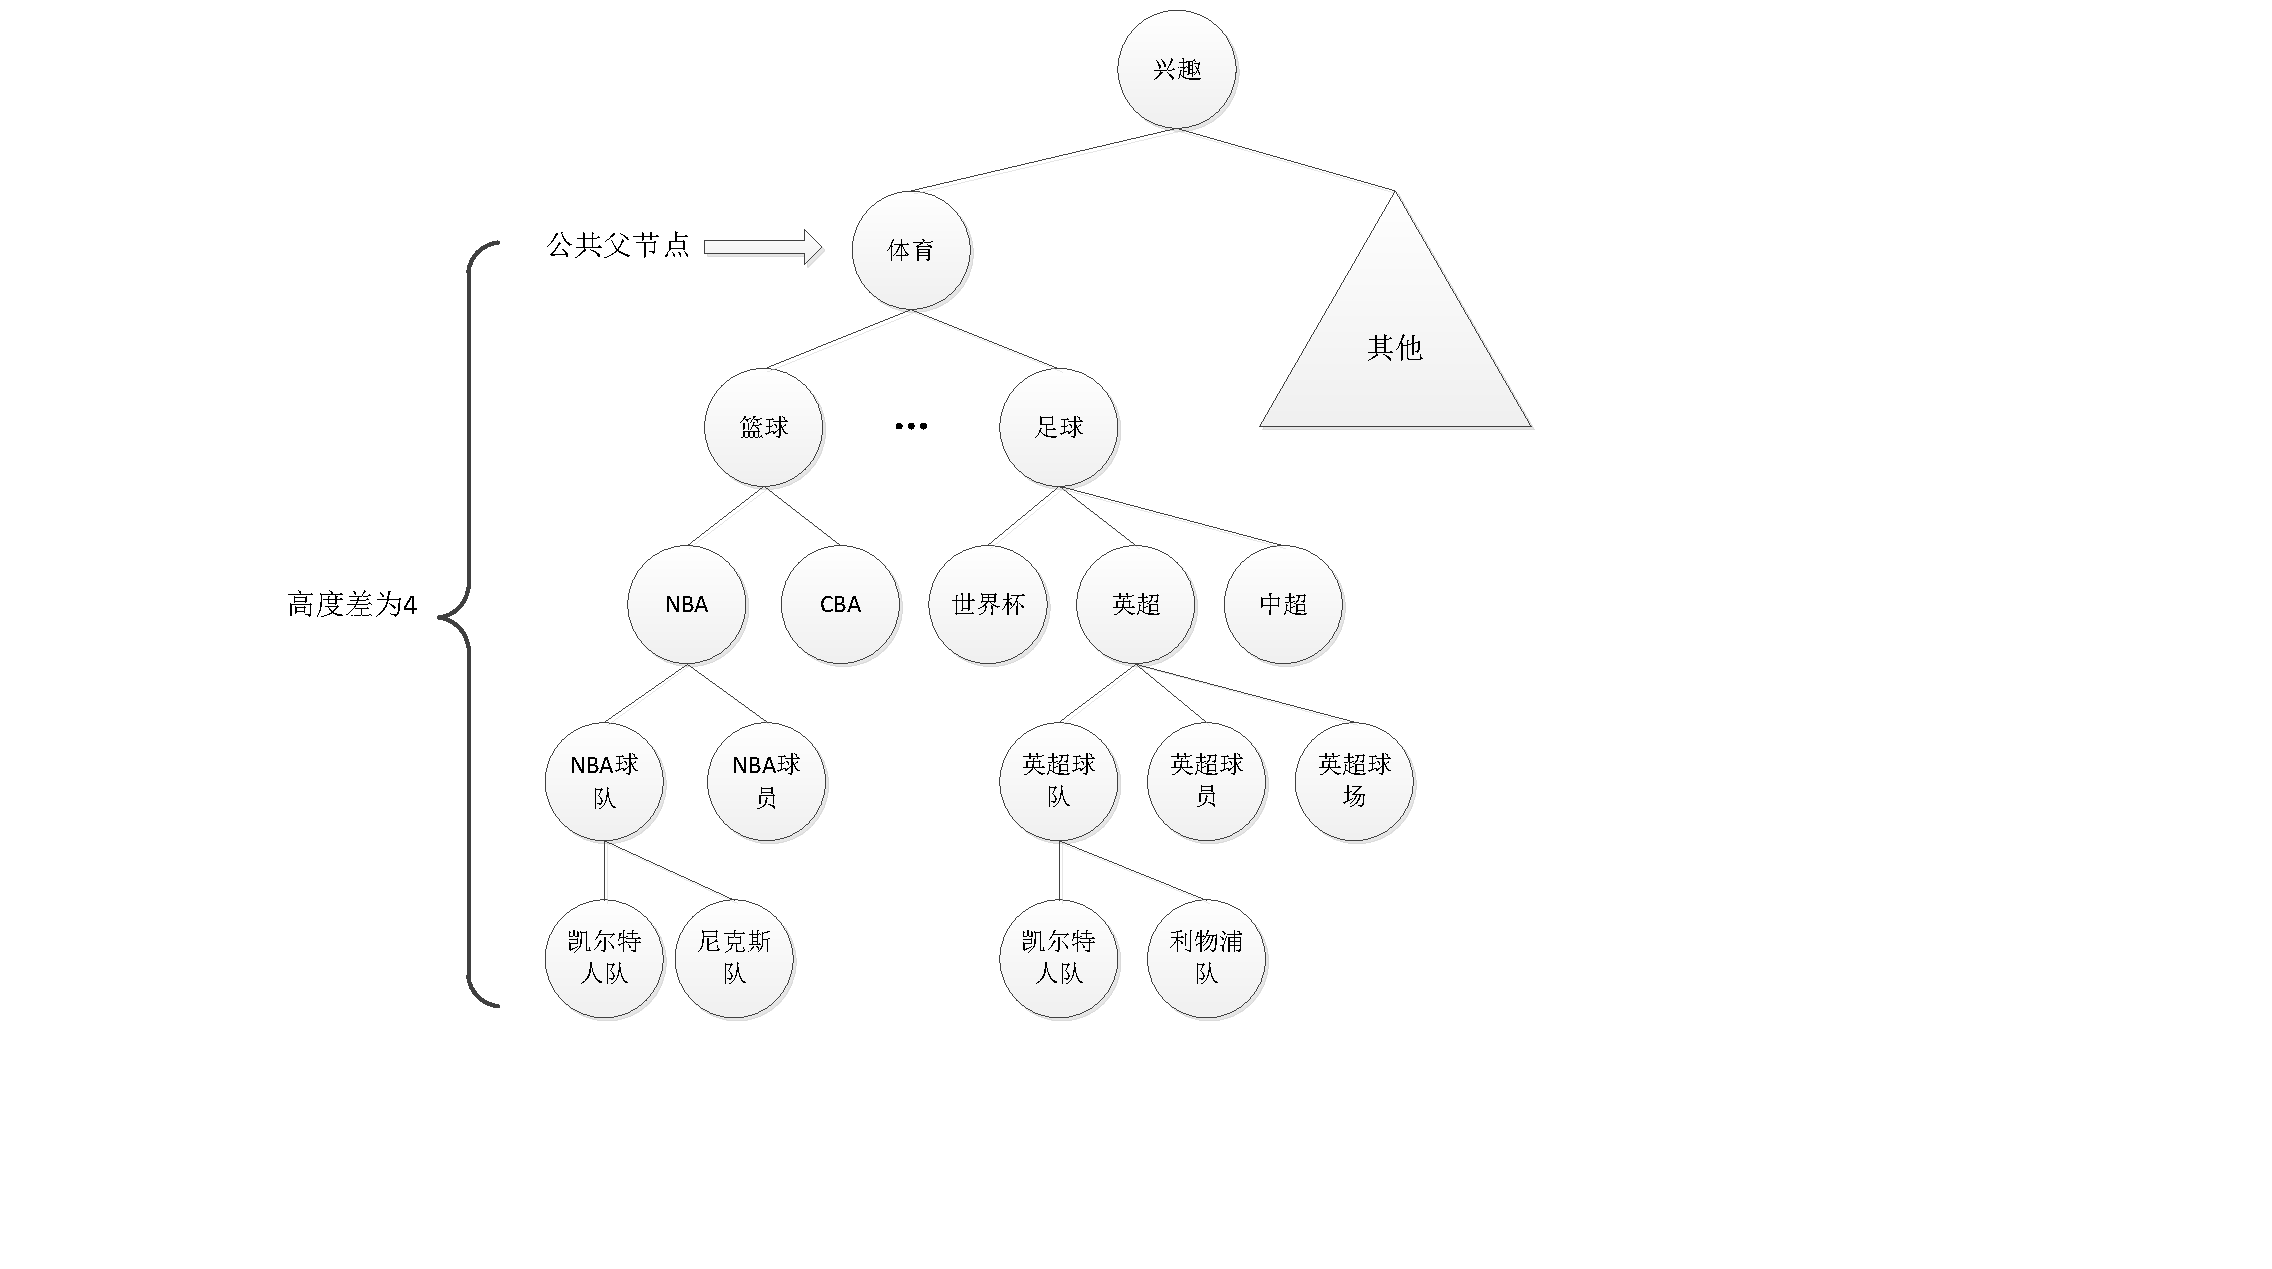
\includegraphics[width=\textwidth]{treeexample.pdf}
\caption{人工构建的一个静态兴趣分类树的实例}
\label{fig:treeexample}
\end{figure}

但是经过仔细思考之后发现,上述假设存在一定的瑕疵。举个反例来说,如图\ref{fig:treeexample}所示的是一种人工构建的可能的静态兴趣分类树。在树中的最底层分别有两个兴趣点都叫做“凯尔特人队”,但是它们一个父节点是“NBA球队”,另一个父节点是“苏超球队”,而且它们的公共父节点是“体育”,距离它们的高度分别都是4,也就是说这两个兴趣点其实差别比较大,于是,按照上述理论得出之间的余弦相似度应该比较小才对。但是事实上,这两个兴趣点的相似度会十分地接近。如表格\ref{tbl:celtics}所示,两个“凯尔特人队”的兴趣点在主题词上的相似性很大,比如“得分”、“防守”、“冠军”等词的权重都非常高。如果仅仅考虑用余弦相似度来计算两者的层次关系时,两者在层次结构上会非常地接近,因此与人工判别的实际情况矛盾。

从而可以看出,仅仅使用余弦相似度来判断兴趣点所在树中的层是存在不足的。所以在条件允许的情况下,使用人工构建的办法来建立一棵全局的静态兴趣分类树是一个更好的办法,主要是保证了层级之间兴趣点的准确性。

\begin{table}[ht]
\caption{“凯尔特人队”兴趣点的向量实例}
\centering
\begin{tabular}{cc|cc} 
\hline
“凯尔特人队(NBA)” & 权值 & “凯尔特人队(苏超)” & 权重 \\
\hline
得分 & 0.131 & 联赛 & 0.201 \\
比赛 & 0.112 & 财务 & 0.098 \\
进攻 & 0.084 & 冠军& 0.082 \\
防守 & 0.048 & 得分 & 0.065 \\
季后赛 & 0.030 & 抽签 & 0.021 \\
首轮 & 0.019 & 防守 & 0.011 \\
击败 & 0.014 & 击败 & 0.007 \\
篮球 & 0.009 & 赞助商 & 0.007 \\
伤病 & 0.003 & 点球 & 0.005 \\
冠军 & 0.001 & 赛事 & 0.002 \\
\hline
\label{tbl:celtics}
\end{tabular}
\end{table}

\subsubsection{基于静态分类树修正的兴趣点匹配}
假设根据一定的办法人工或者半自动地构建出一个全局的静态兴趣分类树后,接下来可以利用这棵树对兴趣点匹配的机制进行修正。在上一节中,已经讨论过直接通过余弦相似度计算出来的兴趣点相似度不能很好反映层级的关系,因此,可以利用已经存在的静态兴趣分类树对兴趣点的相似度在层级关系上进行修正,从而是其更加符合实际情况。

\subsection{动态兴趣伸展树的表示方法}

\subsection{基于用户兴趣的自动推荐方法}

\subsection{小结}
